\subsection*{Questão 09}

\textit{O que indica a fase de um sinal?}\par

\textbf{Resposta:} 
A fase de um sinal, representada pelo ângulo \(\theta\), indica o deslocamento horizontal da onda em relação à origem padrão (tempo \(t=0\)).

Em uma onda senoidal, a fase determina \textbf{quanto a onda está adiantada ou atrasada} no eixo do tempo.
\begin{itemize}
    \item $\theta > 0$: onda adiantada (deslocada para a esquerda)
    \item $\theta < 0$: onda atrasada (deslocada para a direita)
\end{itemize}

\textbf{Exemplo visual: } 
A figura abaixo ilustra duas ondas senoidais com a mesma frequência, mas fases diferentes ($\theta_1=0$ e $\theta_2=\pi/2$), mostrando o deslocamento horizontal entre elas.

\begin{center}
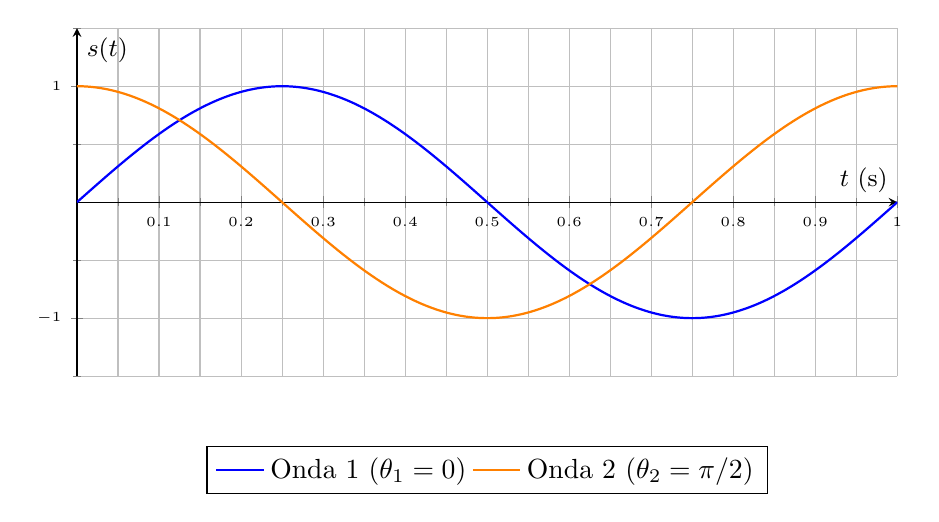
\begin{tikzpicture}
\begin{axis}[
    width=12cm, height=6cm,
    axis lines = middle,
    xlabel = {$t$ (s)},
    ylabel = {$s(t)$},
    label style={font=\small},
    tick label style={font=\tiny},
    grid = both,
    minor tick num = 1,
    domain = 0:1,
    samples = 500,
    xmin=0, xmax=1,
    ymin=-1.5, ymax=1.5,
    legend style={at={(0.5,-0.2)}, anchor=north, legend columns=-1}
]

% Onda 1: fase 0
\addplot [blue, thick] {sin(deg(2 * pi * 1 * x + 0))};
\addlegendentry{Onda 1 ($\theta_1=0$)}

% Onda 2: fase pi/2
\addplot [orange, thick] {sin(deg(2 * pi * 1 * x + pi/2))};
\addlegendentry{Onda 2 ($\theta_2=\pi/2$)}

\end{axis}
\end{tikzpicture}
\end{center}